\documentclass[aspectratio=169]{beamer}
\usepackage{color,amsmath}
\usepackage{subfigure}
\usepackage{booktabs}
\usepackage{framed}
\usepackage{comment}

\def\vf{\vfill}

%%%%%%%%%%%%%%%%%%%%%%%%%%
\title[]{Computer-administered interviews\\and wiki surveys}
\author[]{Matthew J. Salganik\\Department of Sociology\\Princeton University}
\date[]{Summer Institutes in Computational Social Science\\June 20, 2019
\vfill
\begin{flushleft}
{\scriptsize
The Summer Institutes in Computational Social Science is supported by grants from the Russell Sage Foundation and the Alfred P. Sloan Foundation.}
\end{flushleft}
\begin{flushright}

\includegraphics[width=0.1\textwidth]{figures/cc-by.png}
\end{flushright}
}
\begin{document}
%%%%%%%%%%%%%%%%%%%%%%%%%%
\frame{\titlepage}
%%%%%%%%%%%%%%%%%%%%%%%%%%
\begin{frame}

\begin{center}
\small{
\begin{tabular}{ l c c c}
           & Sampling & Interviews & Data environment\\
\hline
1st era & Area probability & Face-to-face & Stand-alone \\
2nd era & \parbox[t]{3cm}{\centering Random digital dial\\probability} & Telephone & Stand-alone \\
3rd era & Non-probability & \textcolor{blue}{Computer-administered} & Linked \\
\end{tabular}
}
\end{center}

\end{frame}
%%%%%%%%%%%%%%%%%%%%%%%%%%%
\begin{frame}

\begin{center}
Human-administered $\rightarrow$ Computer-administered
\end{center}

\begin{itemize}
\item enables change
\item requires change
\end{itemize}

\end{frame}
%%%%%%%%%%%%%%%%%%%%%%%%%%
\begin{frame}
\frametitle{}
\begin{center}
\includegraphics<1>[width=3.5in]{figures/kittenwar_front_1_cut}
\includegraphics<2>[width=3.5in]{figures/kittenwar_front_2_cut}
\includegraphics<3>[width=3.5in]{figures/kittenwar_front_3_cut}
\end{center}
\end{frame}
%%%%%%%%%%%%%%%%%%%%%%%%%%%
\begin{frame}
\begin{center}
\begin{tabular}{ccc}
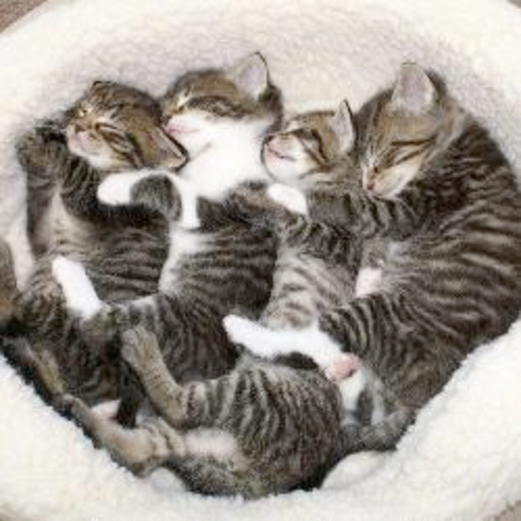
\includegraphics[width=1.2in]{figures/kittenwar_cute_1} & 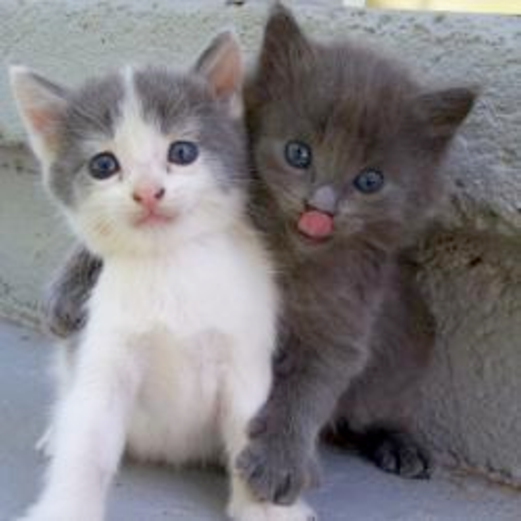
\includegraphics[width=1.2in]{figures/kittenwar_cute_2} & 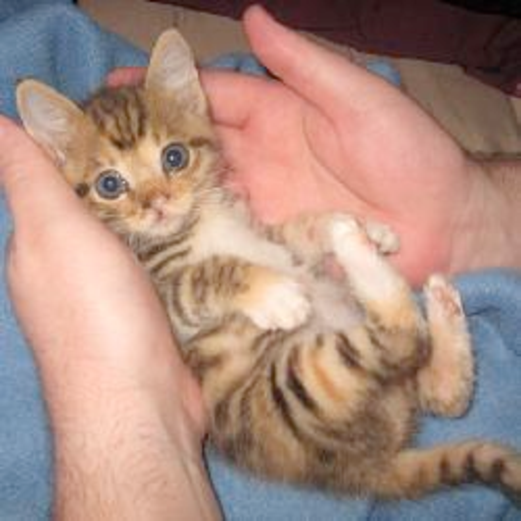
\includegraphics[width=1.2in]{figures/kittenwar_cute_3}\\
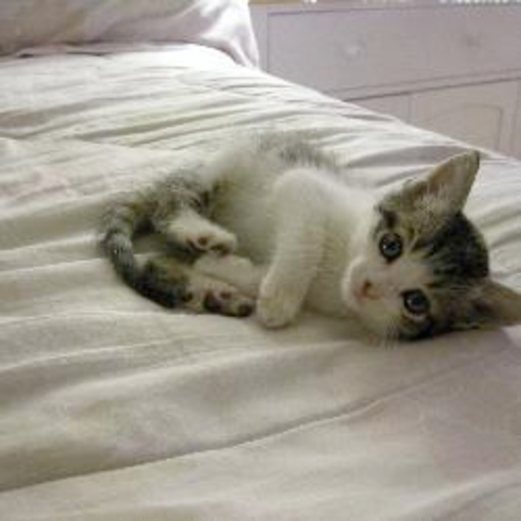
\includegraphics[width=1.2in]{figures/kittenwar_cute_4} & 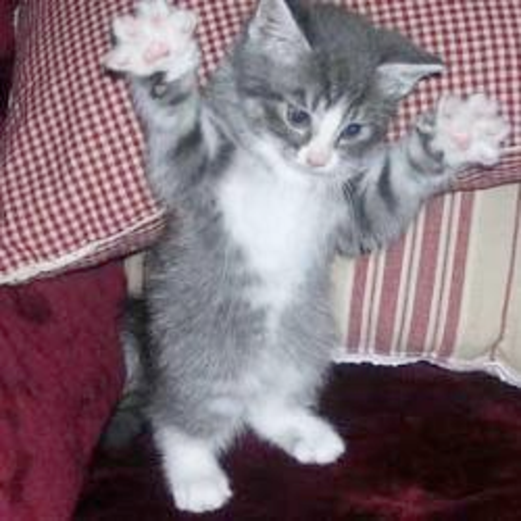
\includegraphics[width=1.2in]{figures/kittenwar_cute_5} & 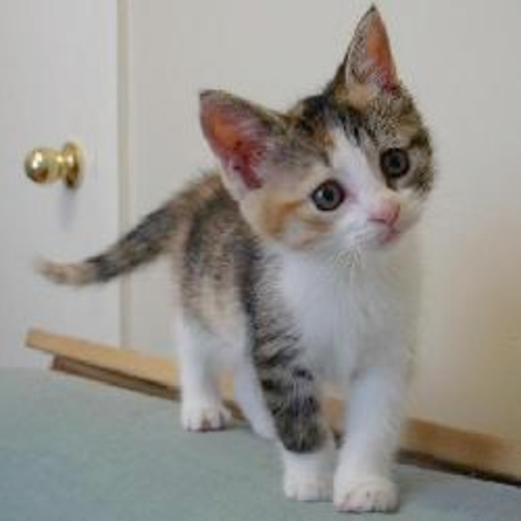
\includegraphics[width=1.2in]{figures/kittenwar_cute_6}
\end{tabular}
\end{center}
\end{frame}
%%%%%%%%%%%%%%%%%%%%%%%%%%%
\begin{frame}
\frametitle{}
\begin{center}
\begin{tabular}{ccc}
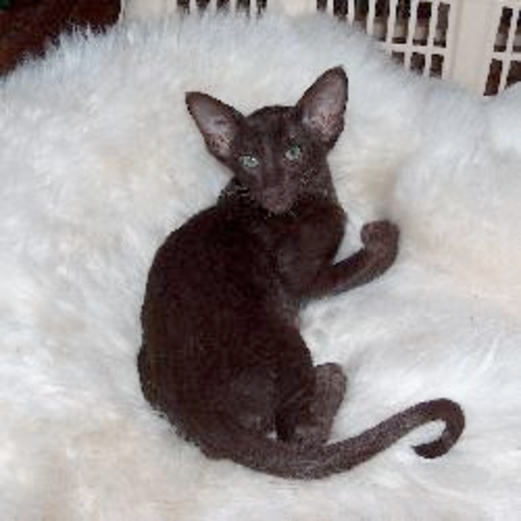
\includegraphics[width=1.2in]{figures/kittenwar_ugly_1} & 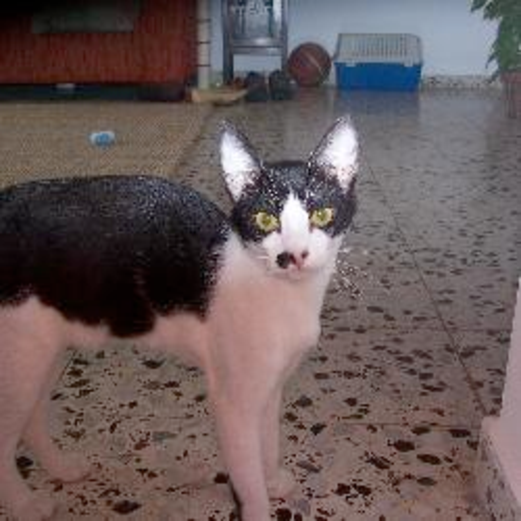
\includegraphics[width=1.2in]{figures/kittenwar_ugly_2} & 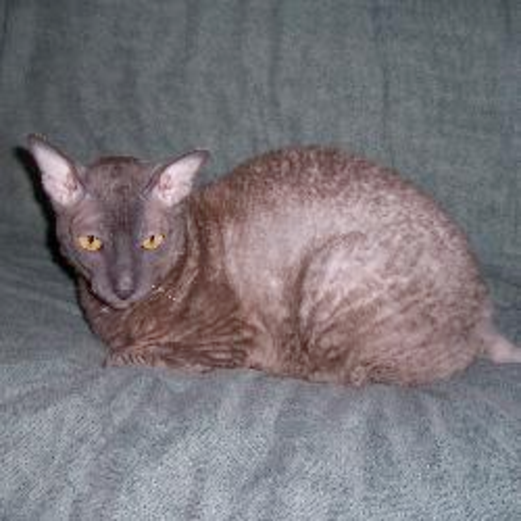
\includegraphics[width=1.2in]{figures/kittenwar_ugly_3}\\
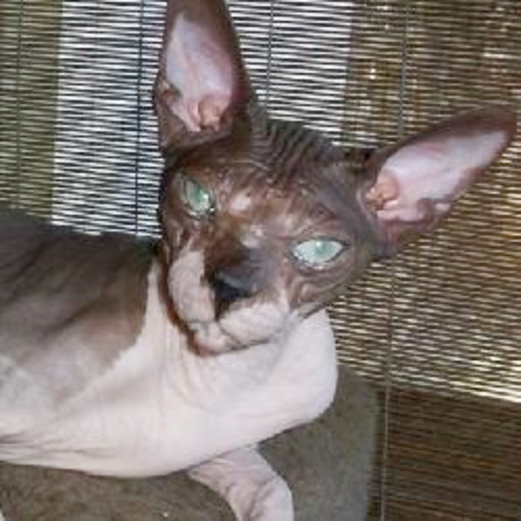
\includegraphics[width=1.2in]{figures/kittenwar_ugly_4} & 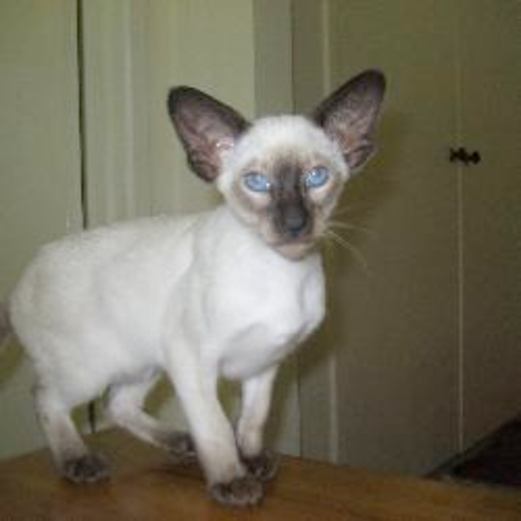
\includegraphics[width=1.2in]{figures/kittenwar_ugly_5} & 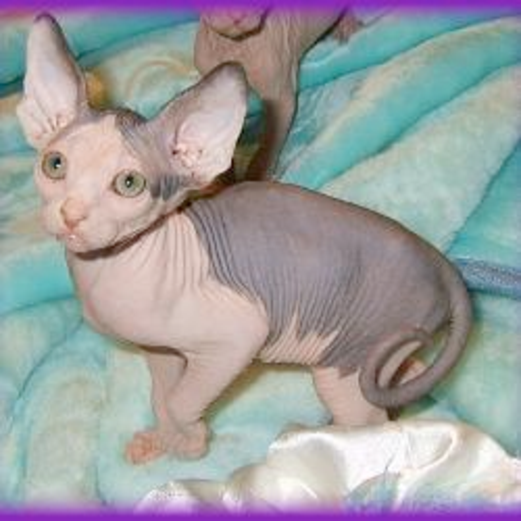
\includegraphics[width=1.2in]{figures/kittenwar_ugly_6}
\end{tabular}
\end{center}
\end{frame}
%%%%%%%%%%%%%%%%%
\begin{frame}

\begin{center}
{\LARGE quantification} or {\LARGE openness} 
\end{center}

\end{frame}
%%%%%%%%%%%%%%%%%
\begin{frame}

\begin{center}
{\LARGE quantification} + {\LARGE openness} =\\ \textcolor{blue}{\LARGE wiki surveys}
\end{center}

\end{frame}
%%%%%%%%%%%%%%%%%%%%%%%%%%
\begin{frame}

General principles of wiki surveys:
\begin{itemize}
\item greedy
\end{itemize}

\end{frame}
%%%%%%%%%%%%%%%%
\begin{frame}

\begin{columns}[c] 
\column{2.5in} 
\hspace{0.6in}Good web-based systems use\\ \hspace{0.6in}the \textcolor{blue}{fat-head} and the \textcolor{blue}{long-tail} 
\column{1in} 
\hspace{-0.3in}
\includegraphics[width=0.6in]{figures/200px-Wikipedia-logo}
\end{columns} 

\begin{center}
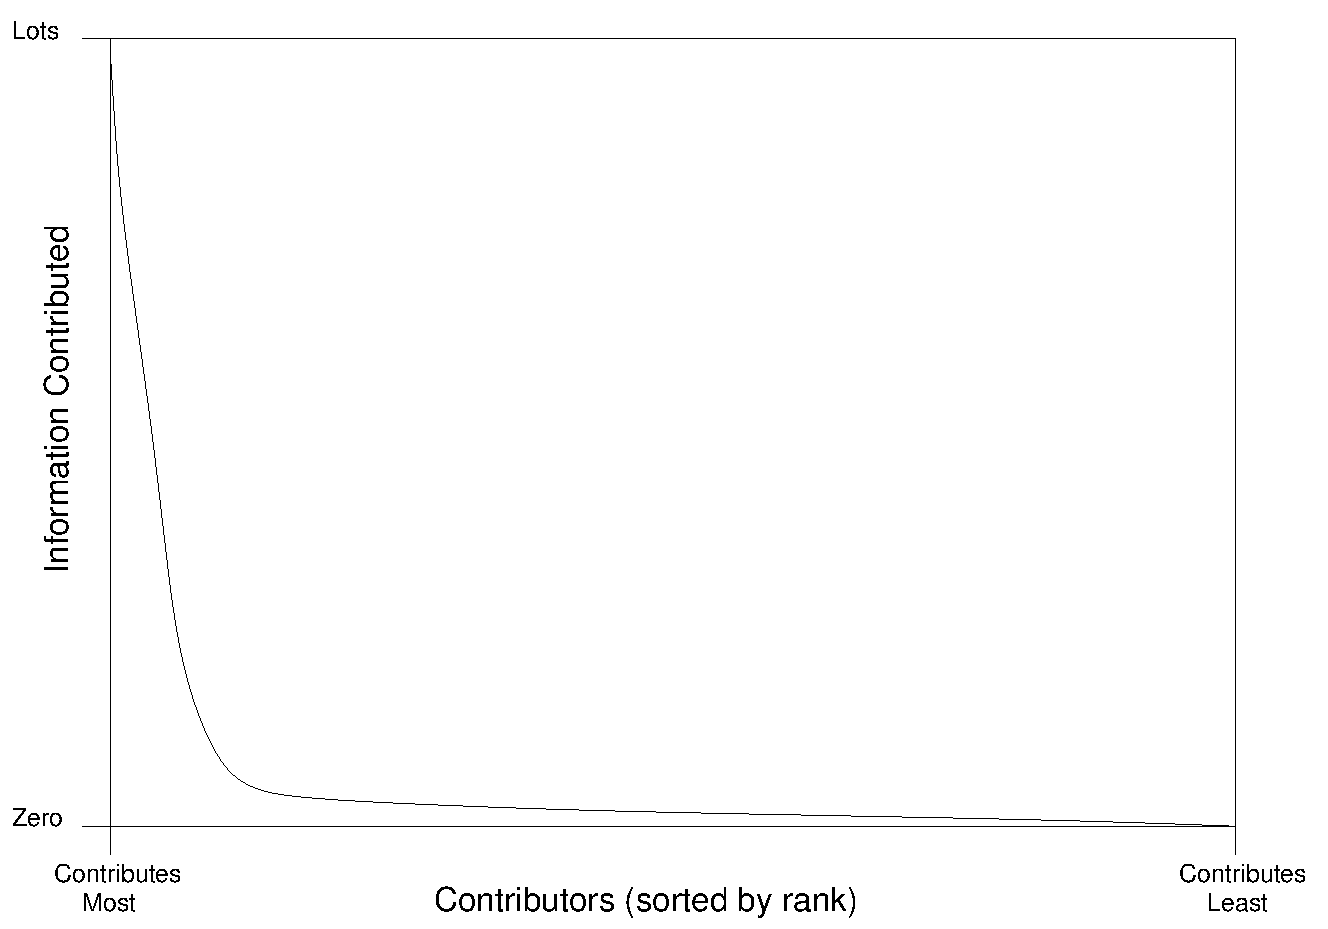
\includegraphics[width=0.7\textwidth]{figures/zipf_plot}
\end{center}

\end{frame}
%%%%%%%%%%%%%%%%%
\begin{frame}

\hspace{0.7in}Surveys don't use the \textcolor{blue}{fat-head} or the \textcolor{blue}{long-tail}

\begin{center}
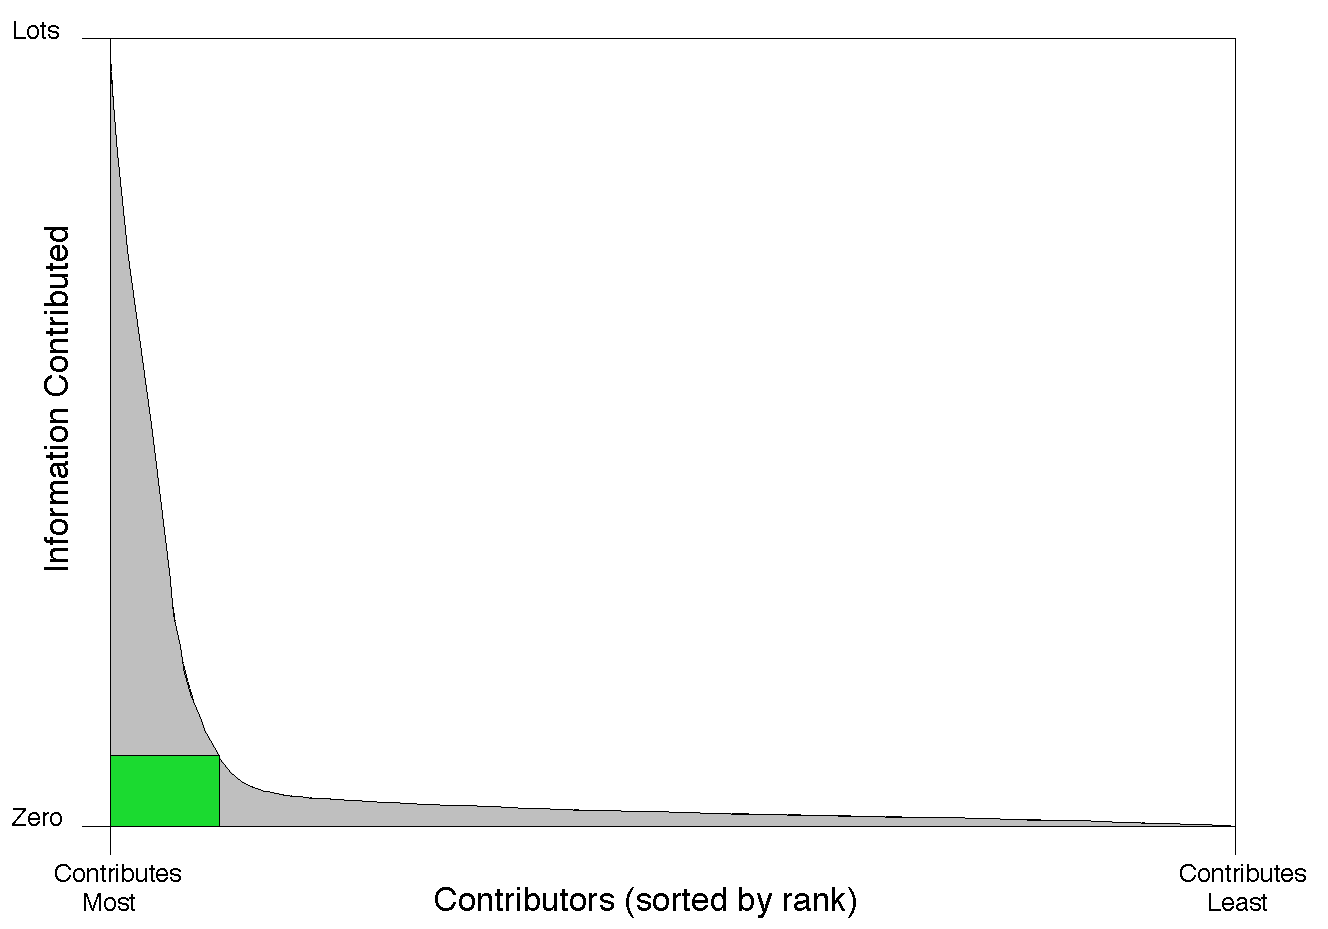
\includegraphics[width=0.8\textwidth]{figures/zipf_plot_withoverlay}
\end{center}

\end{frame}
%%%%%%%%%%%%%%%%%%
\begin{frame}

General principles of wiki surveys:
\begin{itemize}
\item greedy
\pause
\item collaborative
\pause
\item adaptive
\end{itemize}

\end{frame}
%%%%%%%%%%%%%%%%
\begin{frame}

\begin{center}
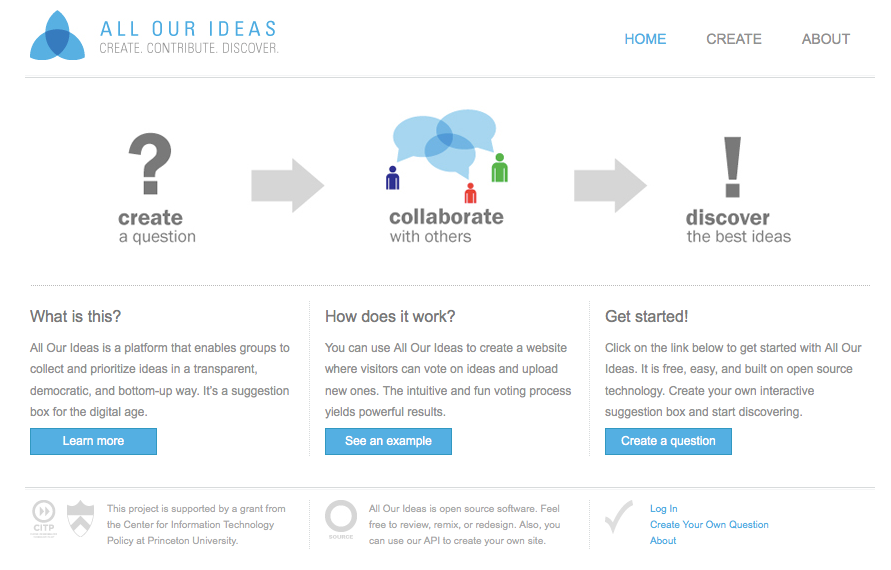
\includegraphics[width=0.9\textwidth]{figures/aoi_splash}
\end{center}

\end{frame}
%%%%%%%%%%%%%%%%%%
\begin{frame}
\frametitle{}

\begin{center}
\includegraphics<1>[width=0.95\textwidth]{figures/planyc_greener_greater}
\end{center}

\end{frame}
%%%%%%%%%%%%%%%%%%%
\begin{frame}
\frametitle{}

\begin{center}
\textcolor{blue}{\large{Which do you think is a better idea for creating a greener, greater New York City?}}\\
\end{center}

Seeded the wiki survey with 25 ideas: 
\begin{itemize}
\item Require all big buildings to make certain energy efficiency upgrades
\item Increase targeted tree plantings in neighborhoods with high asthma rates
\item Establish a New York City Energy Planning Board
\end{itemize}

\end{frame}
%%%%%%%%%%%%%%%%%%%
\begin{frame}

\begin{center}
\includegraphics<1>[width=0.9\textwidth]{figures/planyc_vote1}
\includegraphics<2>[width=0.9\textwidth]{figures/planyc_vote2}
\includegraphics<3>[width=0.9\textwidth]{figures/planyc_vote3}
\end{center}

\end{frame}
%%%%%%%%%%%%%%%%%
\begin{frame}

\begin{center}
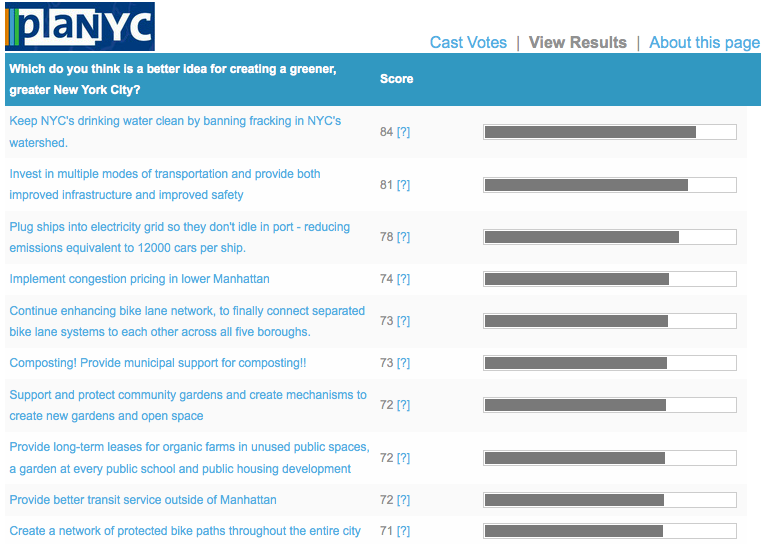
\includegraphics[width=0.8\textwidth]{figures/planyc_results}
\end{center}

\end{frame}
%%%%%%%%%%%%%%%%%%
%\begin{frame}
%
%\begin{center}
%\includegraphics[width=\textwidth]{figures/aoi_schematic}
%\end{center}
%
%\end{frame}
%%%%%%%%%%%%%%%%%
%\begin{frame}
%\frametitle{Suggestions for Princeton student government}
%
%\begin{itemize}
%\item 2,000 participants  (40\% of undergrads)
%\item 40,000 votes
%\item 100 new ideas
%\end{itemize}
%$\rightarrow$ Two of the top five ideas were uploaded by students
%\end{frame}

%%%%%%%%%%%%%%%%%
\begin{frame}
\frametitle{What are we trying to estimate?}

\begin{columns}[t] % the "c" option specifies center vertical alignment

\column{0.45\textwidth} % column designated by a command
\begin{center}
\textcolor{blue}{Data}
\end{center}
\begin{tabular}{cccc}
\toprule
\footnotesize{Vote} & \footnotesize{Session} & \multicolumn{2}{c}{\footnotesize{Prompt}} \\
\midrule
\footnotesize{1} & \footnotesize{1} & \textbf{\footnotesize{item 4}} & \footnotesize{item 1}\\
\footnotesize{2} & \footnotesize{1} & \footnotesize{item 3} & \textbf{\footnotesize{item 1}} \\
\footnotesize{3} & \footnotesize{1} & \textbf{\footnotesize{item 4}} & \footnotesize{item 3} \\
\footnotesize{4} & \footnotesize{2} & \textbf{\footnotesize{item 3}} & \footnotesize{item 4} \\ 
\footnotesize{5} & \footnotesize{2} & \footnotesize{item 4} & \textbf{\footnotesize{item 2}} \\
\vdots & \vdots & \vdots & \vdots\\
\bottomrule
\end{tabular}

\column{0.1\textwidth}
\vskip 5em
\begin{center}

\includegraphics{figures/green_arrow}
\end{center}

\column{0.40\textwidth}
\begin{center}
\textcolor{blue}{Opinion matrix}
\end{center}
%\large
$\left[
\begin{array}{cccc}
\theta_{1,1} & \theta_{1,2} & \ldots & \theta_{1,K} \\
\theta_{2,1} & \theta_{2,2} & \ldots & \theta_{2,K} \\
\vdots & \vdots & \ddots & \vdots\\
\theta_{J,1} & \theta_{J,2} & \ldots & \theta_{J,K} \\
\end{array} 
\right]
$
%}
\vskip 1em
$\theta_{j,k}$: how much respondent $j$ likes item $k$ 
\end{columns}

\end{frame}
%%%%%%%%%%%%%%%%%
\begin{comment}
\begin{frame}
\frametitle{What are we trying to estimate?}

\begin{itemize}
\item What are the ideas with highest overall support?
\item What are the ideas with the most variability in support (i.e., most polarizing)?
\item Which ideas are most similar to each other?
\end{itemize}
If we have information about the demographics of the people (age, level of education, gender, race/ethinicty, etc.)
\begin{itemize}
\item What ideas are the most polarizing across groups?
\item Which demographics more strongly predict opinions about which ideas?
\end{itemize}

\end{frame}
\end{comment}
%%%%%%%%%%%
\begin{frame}
\frametitle{}

\begin{center}
\textcolor{blue}{\large{Which do you think is a better idea for creating a greener, greater New York City?}}\\
\end{center}

Seeded the wiki survey with 25 ideas: 
\begin{itemize}
\item Require all big buildings to make certain energy efficiency upgrades
\item Increase targeted tree plantings in neighborhoods with high asthma rates
\item Establish a New York City Energy Planning Board
\end{itemize}

\end{frame}
%%%%%%%%%%%%%%%%%%%
\begin{frame}
\frametitle{}

Recruited participants through Twitter, Facebook, blogs, etc. 
\begin{center}
\includegraphics<1>[width=\textwidth]{figures/planyc_tweet}
\end{center}

This is \textcolor{blue}{not a random sample}, but random samples are possible
\end{frame}
%%%%%%%%%%%%%%%%%%
\begin{frame}

\begin{itemize}
\item 31,893 responses
\item 464 ideas uploaded 
\end{itemize}

\begin{center}
\includegraphics<1>[width=0.7\textheight]{figures/planyc_user_activity_responses}
\end{center}

\end{frame}
%%%%%%%%%%%%%%%%%%
\begin{frame}
\frametitle{}

\begin{center}
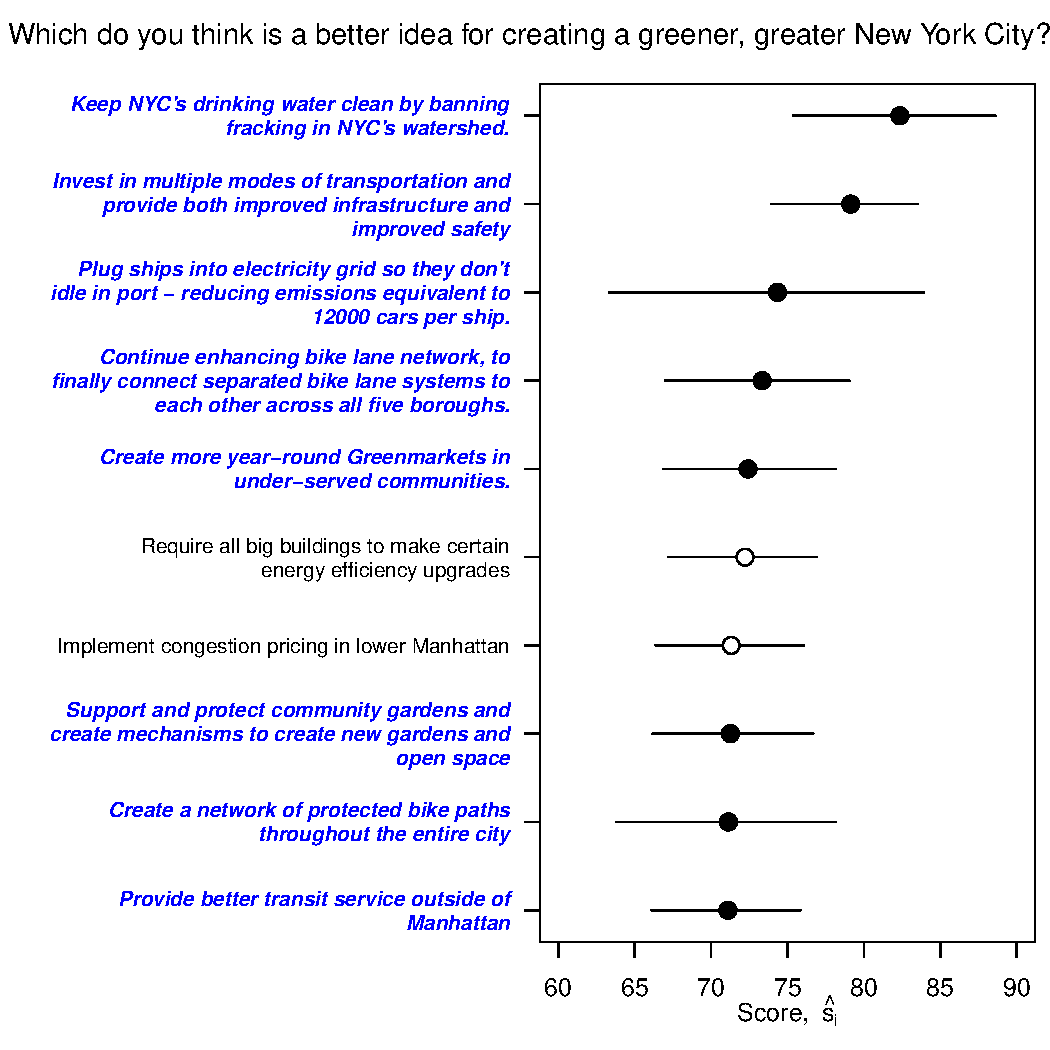
\includegraphics[width=0.96\textheight]{figures/planyc_sigma1_top10_blue}
\end{center}

\end{frame}
%%%%%%%%%%%%%%%%%%
\begin{frame}
\frametitle{}

\begin{itemize}
\item Alternative framings: \textcolor{blue}{``Keep NYC's drinking water clean by banning fracking in NYC's watershed''}
\pause
\item Novel information: \textcolor{blue}{``Plug ships into electricity grid so they don't idle in port - reducing emissions equivalent to 12000 cars per ship.''}
\end{itemize}

\end{frame}
%%%%%%%%%%%%%%%%%
\begin{frame}

\begin{center}
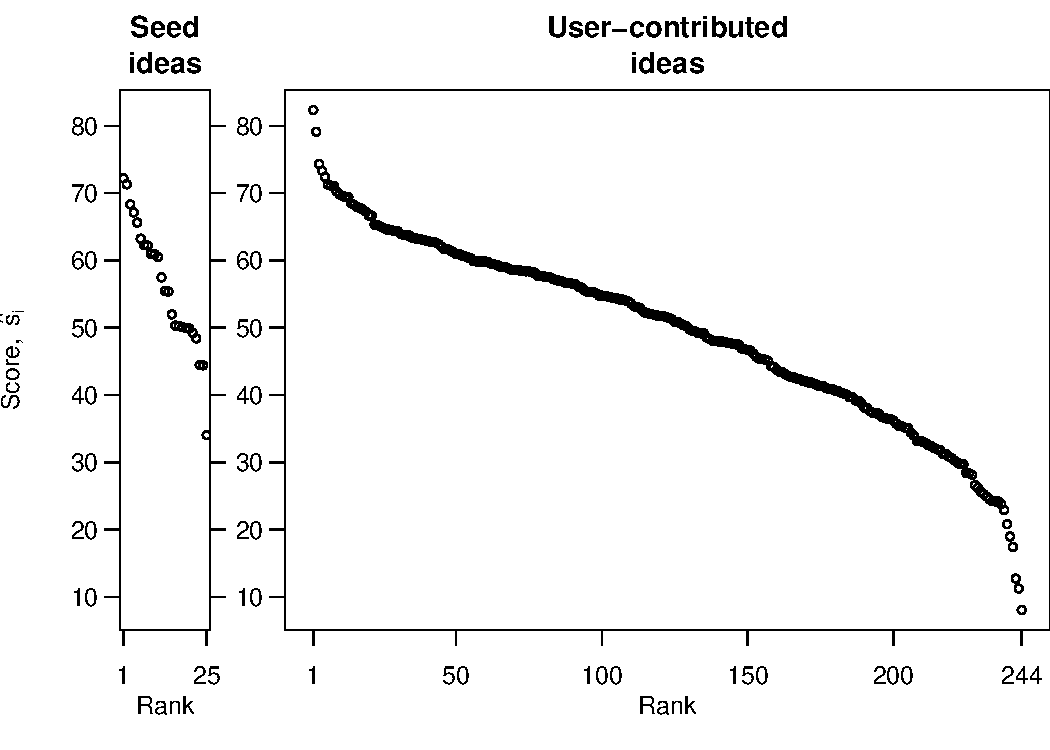
\includegraphics[width=0.65\textwidth]{figures/planyc_sigma1_compare_seed_user-contributed}
\end{center}

\pause
\Large{
\begin{center}
$\mbox{variance} + \mbox{volume} \rightarrow \mbox{extreme cases}$ 
\end{center}
}

\end{frame}
%%%%%%%%%%%%%%%%
\begin{frame}

\begin{center}
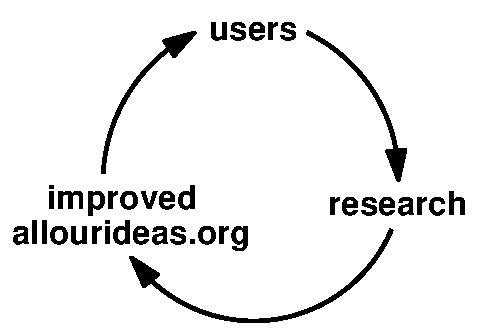
\includegraphics[width=0.6\textwidth]{figures/virtuous_cycle}
\end{center}

\end{frame}
%%%%%%%%%%%%%%%%
\begin{frame}

Currently hosting:\\
14,000 wiki surveys with 75,000 ideas and 23 million votes
\vf

\begin{center}
\begin{tabular}{m{1.4in} m{1.4in} m{1.4in}}

\includegraphics[width=1.2in]{figures/edemocracia} & 
\includegraphics[width=1.4in]{figures/ows_horizontal} & 
\includegraphics[width=1.3in]{figures/legg_mason_logo}\\
\vspace{0.2in}

\includegraphics[width=1.1in]{figures/un_logo_white_bkg} & 
\includegraphics[width=1in]{figures/200px-Wikipedia-logo} & 
\includegraphics[width=1.2in]{figures/harvard_business_publishing}
\end{tabular}
\end{center}

\end{frame}
%%%%%%%%%%%%%%%%%
\begin{frame}

\begin{itemize}
\item Questions about building it?
\item Questions about system-building as part of social research? (professional concerns?, kinds of things learned?)
\end{itemize}

\end{frame}
%%%%%%%%%%%%%%%%%


\end{document}
